The analysis of the results produced by our code passed through a series of intermediate and progressive steps, continuously checking the outcomes obtained via the simulation with the analytical formulas, fortunately available for the non-interacting case. We will now proceed with the presentation of the results derived within the context of our project, enlightening the features of any performed simulation and the methods to validate the solidity and efficiency of the code. First we will focus on the runs carried out in non-interacting case both with the brute-force Metropolis algorithm and the importance sampling, proceeding then towards a more detailed statistical analysis through the blocking method. Then the interaction between particles will be introduced, together with the gradient descent method for the research of the $\alpha$ which minimizes the energy and then concluding with the one-body density evaluation.


\subsection{NON-INTERACTING SYMMETRICAL CASE}
\subsubsection{BRUTE-FORCE METROPOLIS ALGORITHM}
At first we chose a spherical potential trap with a simple gaussian trial wavefunction, these obtained by setting $a=0$ and $\beta=\omega_z=1$ into Eq.\,\ref{potential} and Eq.\,\ref{wavefunctions}. In order to obtain a numerical estimation of the ground state energy of the system we first adopted the so called Brute-Force Metropolis algorithm, previously introduced. We performed different simulations varying many parameters of the system and before each of these runs the system was submitted to $10^5$ thermalization steps. This choice has been preserved for each simulation presented from now on in the report. In principle we could have reduced the number of thermalization steps for the most simple configurations, involving for example 1 particles in a 1-dimensional system. However, since the most time-demanding operation is the evaluation of the local energy (not performed for the thermalization steps), the computational time for the initialization is considerably low, even with such an amount of steps and a large number of particles. We notice also that with the highest number of particles adopted for the system ($N=500$), within a $10^5$-steps thermalization process each of them will on average be moved 200 times, reasonably sufficient for Markov chain to converge to the stationary PDF. \\

Table \ref{tab:tab_x_metropolis_analytical} reports the results of the analysis of the system's dependence on the number of particles and dimension. The value of $\alpha$ was kept fixed at $\alpha^{best} = 0.5$. The corresponding results obtained using the numerical method to evaluate the second derivative are reported in Table \ref{tab:tab_x_metropolis_numerical}. One can immediately notice a significant increase in the simulation time with the numerical approach, hence leaving the only purpose of this second method to perform preliminary tests and qualitative studies. Proceeding, Figure \ref{fig:varying_alpha_noninteract_metropolis}, shows the value of the ground state energy of the system as a function of the parameter $\alpha$ for a particular configuration of the simulation settings, that is $N=10$ particles, 3 dimensions, $2^{21}$ steps and Metropolis step-size $r_{step} = 1.0$. One can immediately notice that the function is convex, which guarantees the existence of one unique minimum point, in accordance to what discussed in the context of the gradient descent method. In this simple case, the convexity of the energy curve as a function of $\alpha$ was expected, as it can be derived from the analytical form available in Eq.\,\ref{energy_analitical}. Some selected results for different $\alpha$ values are reported also in Table \ref{tab:varying_alpha_noninteracting}, referring to simulations performed again for a $3D$ system with $N=10$ and $N_{steps}=2^{21}$. This table contains also a comparison between the variance calculated as $\sigma^2_E = \left\langle E_L^2 \right\rangle - \left\langle E_L \right\rangle^2$ and the variance calculated via the blocking method as explained in Section \ref{sec:blocking_method}.

\begin{table}[H]
    \centering
    \begin{tabular}{cccccc}
    $N_{part}$ & $N_{dim}$ & $\langle E_L \rangle$ & $\sigma^2_E$ & $t_{CPU}$ & acc. ratio \\
    \midrule
    1 & 1 & 0.50000 & 0.00000 & 0 & 0.5 \\
    1 & 2 & 1.0000 & 0.00000 & 0 & 0.5 \\
    1 & 3 & 1.5000 & 0.00000 & 0 & 0.5 \\
    \midrule
    10 & 1 & 5.0000 & 0.00000 & 0 & 0.5 \\
    10 & 2 & 10.000 & 0.00000 & 0 & 0.5 \\
    10 & 3 & 15.000 & 0.00000 & 0 & 0.5 \\
    \midrule
    50 & 1 & 25.000 & 0.00000 & 0 & 0.5 \\
    50 & 2 & 50.000 & 0.00000 & 0 & 0.5 \\
    50 & 3 & 75.000 & 0.00000 & 0 & 0.5 \\
    \midrule
    100 & 1 & 50.000 & 0.00000 & 0 & 0.5 \\
    100 & 2 & 100.00 & 0.00000 & 0 & 0.5 \\
    100 & 3 & 150.00 & 0.00000 & 0 & 0.5 \\
    \midrule
    500 & 1 & 250.00 & 0.00000 & 0 & 0.5 \\
    500 & 2 & 500.00 & 0.00000 & 0 & 0.5 \\
    500 & 3 & 750.00 & 0.00000 & 0 & 0.5 \\
    \bottomrule
    \end{tabular}
    \caption{The table reports the results of the simulations of the non-interacting case using a simple gaussian trial wavefunction and a brute-force Metropolis sampling method with $N_{steps}=2^{21}$, step-size set to $r_{step}=1.0$ and constant value for $\alpha^{best}=0.5$. The local energy is evaluated exploiting the analytical formula and $\sigma_E^2$ is the variance of the $E_L$ samples generated during the run. }
    \label{tab:tab_x_metropolis_analytical}
\end{table}

\begin{table}[H]
    \centering
    \begin{tabular}{cccccc}
    $N_{part}$ & $N_{dim}$ & $\langle E_L \rangle $ & $\sigma^2_E$ & $t_{CPU}$ & acc. ratio \\
    \midrule
    1 & 1 & 0.50000 & 0.00000 & 0 & 0.5 \\
    1 & 2 & 1.0000 & 0.00000 & 0 & 0.5 \\
    1 & 3 & 1.5000 & 0.00000 & 0 & 0.5 \\
    \midrule
    10 & 1 & 5.0000 & 0.00000 & 0 & 0.5 \\
    10 & 2 & 10.000 & 0.00000 & 0 & 0.5 \\
    10 & 3 & 15.000 & 0.00000 & 0 & 0.5 \\
    \midrule
    50 & 1 & 25.000 & 0.00000 & 0 & 0.5 \\
    50 & 2 & 50.000 & 0.00000 & 0 & 0.5 \\
    50 & 3 & 75.000 & 0.00000 & 0 & 0.5 \\
    \midrule
    100 & 1 & 50.000 & 0.00000 & 0 & 0.5 \\
    100 & 2 & 100.00 & 0.00000 & 0 & 0.5 \\
    100 & 3 & 150.00 & 0.00000 & 0 & 0.5 \\
    \midrule
    500 & 1 & 250.00 & 0.00000 & 0 & 0.5 \\
    500 & 2 & 500.00 & 0.00000 & 0 & 0.5 \\
    500 & 3 & 750.00 & 0.00000 & 0 & 0.5 \\
    \bottomrule
    \end{tabular}
    \caption{The table reports the results of the simulations of the non-interacting case using a simple gaussian trial wavefunction and a brute-force Metropolis sampling method with $N_{steps}=2^{21}$, step-size set to $r_{step}=1.0$ and constant value for $\alpha^{best}=0.5$. The local energy is evaluated exploiting the numerical second derivative and $\sigma_E^2$ is the variance of the $E_L$ samples generated during the run. }
    \label{tab:tab_x_metropolis_numerical}
\end{table}

\begin{figure}[H]
    \centering
    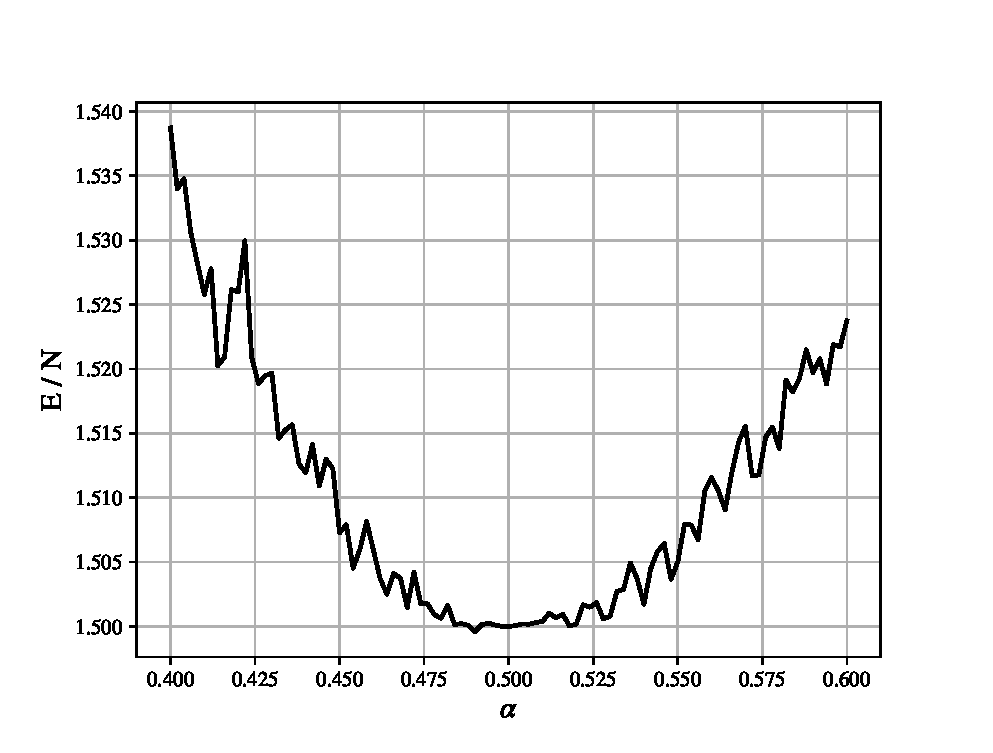
\includegraphics[scale=0.5]{images/varying_alpha_noninteract.eps}
    \caption{The figure reports the energy estimates as a function of $\alpha$ generated by various VMC simulations exploiting the brute-force Metropolis algorithm with $N_{steps}=2^{21}$ and $r_{step}=1$. The curve is referred to a $3D$ system with $N=10$ non-interacting particles. }
    \label{fig:varying_alpha_noninteract_metropolis}
\end{figure}


\subsubsection{IMPORTANCE SAMPLING}
The immediate improvement of this simple model was the inclusion of the importance sampling. This allowed us to bias the random walk in the configuration space according to the probability distribution, leading thus to higher number of accepted steps in the Monte Carlo run. Note that since the particles are now biased to move towards region of higher probability (i.e. the origin), more Monte Carlo cycles are required to find the particles far enough from the origin to obtain a significant result. As for the Brute Force Metropolis, results for fixed $\alpha=0.5$ obtained with the analytical and numerical evaluation of the local energy are reported respectively in Table \ref{tab:tab_x_importance_analytical} and Table \ref{tab:tab_x_importance_numerical}. The estimated energy as a function of $\alpha$ for a $3D$ system populated by 10 particles is reported in Figure \ref{fig:varying_alpha_noninteract_importance} with some selected results in Table \ref{tab:varying_alpha_noninteracting}. All the simulations cited above have been carried out with $2^{21}$ Monte Carlo steps and $\delta t = 0.01$.


\begin{table}[H]
    \centering
    \begin{tabular}{cccccc}
    $N_{part}$ & $N_{dim}$ & $\langle E_L \rangle$ & $\sigma^2_E$ & $t_{CPU}$ & acc. ratio \\
    \midrule
    1 & 1 & 0.50000 & 0.00000 & 0 & 0.5 \\
    1 & 2 & 1.0000 & 0.00000 & 0 & 0.5 \\
    1 & 3 & 1.5000 & 0.00000 & 0 & 0.5 \\
    \midrule
    10 & 1 & 5.0000 & 0.00000 & 0 & 0.5 \\
    10 & 2 & 10.000 & 0.00000 & 0 & 0.5 \\
    10 & 3 & 15.000 & 0.00000 & 0 & 0.5 \\
    \midrule
    50 & 1 & 25.000 & 0.00000 & 0 & 0.5 \\
    50 & 2 & 50.000 & 0.00000 & 0 & 0.5 \\
    50 & 3 & 75.000 & 0.00000 & 0 & 0.5 \\
    \midrule
    100 & 1 & 50.000 & 0.00000 & 0 & 0.5 \\
    100 & 2 & 100.00 & 0.00000 & 0 & 0.5 \\
    100 & 3 & 150.00 & 0.00000 & 0 & 0.5 \\
    \midrule
    500 & 1 & 250.00 & 0.00000 & 0 & 0.5 \\
    500 & 2 & 500.00 & 0.00000 & 0 & 0.5 \\
    500 & 3 & 750.00 & 0.00000 & 0 & 0.5 \\
    \bottomrule
    \end{tabular}
    \caption{The table reports the results of the simulations of the non-interacting case using a simple gaussian trial wavefunction and the importance sampling method with $N_{steps}=2^{21}$, $\delta t = 0.01$ and constant value for $\alpha^{best}=0.5$. The local energy is evaluated exploiting the analytical formula and $\sigma_E^2$ is the variance of the $E_L$ samples generated during the run. }
    \label{tab:tab_x_importance_analytical}
\end{table}

\begin{table}[H]
    \centering
    \begin{tabular}{cccccc}
    $N_{part}$ & $N_{dim}$ & $\langle E_L \rangle$ & $\sigma^2_E$ & $t_{CPU}$ & acc. ratio \\
    \midrule
    1 & 1 & 0.50000 & 0.00000 & 0 & 0.5 \\
    1 & 2 & 1.0000 & 0.00000 & 0 & 0.5 \\
    1 & 3 & 1.5000 & 0.00000 & 0 & 0.5 \\
    \midrule
    10 & 1 & 5.0000 & 0.00000 & 0 & 0.5 \\
    10 & 2 & 10.000 & 0.00000 & 0 & 0.5 \\
    10 & 3 & 15.000 & 0.00000 & 0 & 0.5 \\
    \midrule
    50 & 1 & 25.000 & 0.00000 & 0 & 0.5 \\
    50 & 2 & 50.000 & 0.00000 & 0 & 0.5 \\
    50 & 3 & 75.000 & 0.00000 & 0 & 0.5 \\
    \midrule
    100 & 1 & 50.000 & 0.00000 & 0 & 0.5 \\
    100 & 2 & 100.00 & 0.00000 & 0 & 0.5 \\
    100 & 3 & 150.00 & 0.00000 & 0 & 0.5 \\
    \midrule
    500 & 1 & 250.00 & 0.00000 & 0 & 0.5 \\
    500 & 2 & 500.00 & 0.00000 & 0 & 0.5 \\
    500 & 3 & 750.00 & 0.00000 & 0 & 0.5 \\
    \bottomrule
    \end{tabular}
    \caption{The table reports the results of the simulations of the non-interacting case using a simple gaussian trial wavefunction and the importance sampling method with $\delta t = 0.01$ and constant value for  $\alpha^{best}=0.5$. The local energy is evaluated exploiting the numerical second derivative and $\sigma_E^2$ is the variance of the $E_L$ samples generated during the run. }
    \label{tab:tab_x_importance_numerical}
\end{table}

\begin{figure}[H]
    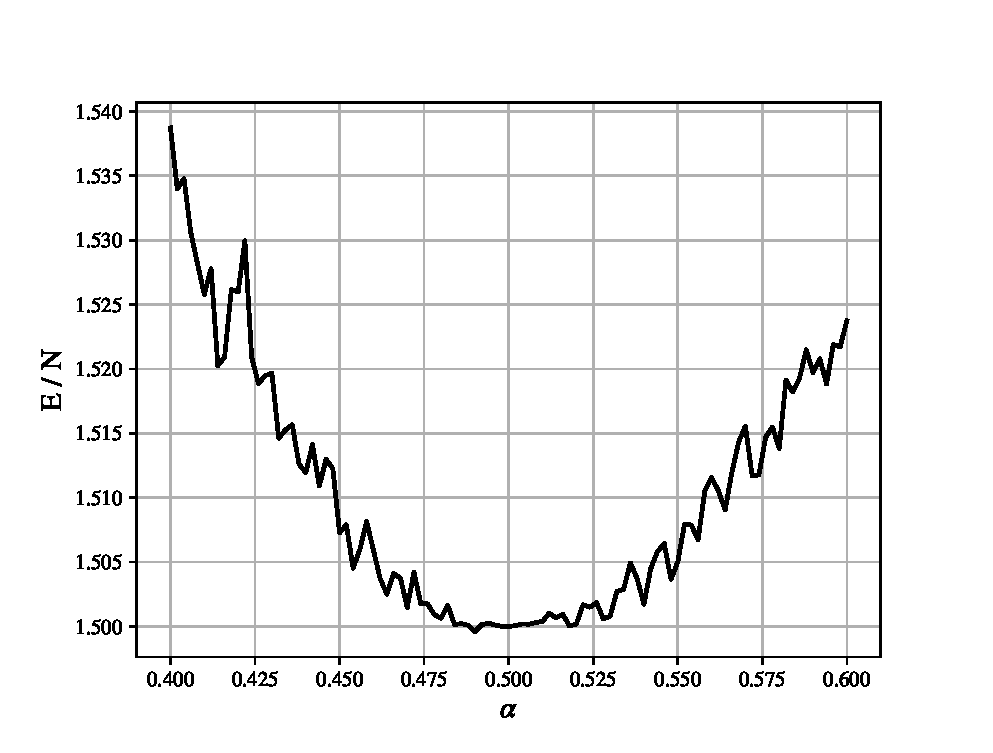
\includegraphics[scale=0.5]{images/varying_alpha_noninteract.eps}
    \caption{The figure reports the energy estimates as a function of $\alpha$ generated by various VMC simulations exploiting the importance sampling with $N_{steps}=2^{21}$, $\delta t = 0.01$. The curve is referred to a $3D$ system with $N=10$ non-interacting particles.}
    \label{fig:varying_alpha_noninteract_importance}
\end{figure}


\begin{table}[H]
    \centering
    \begin{tabular}{c|ccc|ccc}
         & \multicolumn{3}{c|}{Metropolis} & \multicolumn{3}{c}{Importance Sampling} \\
        \midrule
         $\alpha$ & $\langle E_L \rangle$ & $\sigma^2_E/N$ & $\sigma^2_B$ & $\langle E_L \rangle$ & $\sigma^2_E/N$ & $\sigma^2_B$ \\
         \midrule
         $0.3$ & $0$ & $0$ & $0$ & $0$  & $0$ & $0$ \\
         $0.4$ & $0$ & $0$ & $0$ & $0$  & $0$ & $0$ \\
         $0.5$ & $0$ & $0$ & $0$ & $0$  & $0$ & $0$ \\
         $0.6$ & $0$ & $0$ & $0$ & $0$  & $0$ & $0$ \\
         $0.7$ & $0$ & $0$ & $0$ & $0$  & $0$ & $0$ \\
         \bottomrule
    \end{tabular}
    \caption{Results of the simulations for different values of the variational parameter $\alpha$. Here $\sigma_E^2$ and $\sigma_B^2$ refer to the variance estimated respectively on the whole set of $E_L$ values and with the blocking analysis. For both the brute-force Metropolis case and the Importance Sampling case we used 10 particles in 3 dimensions and $2^{21}$ steps. The chosen step-size for the Metropolis algorithm was $r_{step}=1.0$ and the time step-size for the Importance Sampling was $\delta t = 0.01$. }
    \label{tab:varying_alpha_noninteracting}
\end{table}

Even if simple and primitive, this model allowed us to test many of the fundamental parts of the code and made us understand how to fine-tune some parameters involved in the problem. For example, we analysed the effects of the time-step length $\delta t$ in the importance sampling case (see figure \ref{fig:dt_importance_sampling}), concluding that a good choice for the parameter could be $\delta t = 0.01$. Our choice is justified by the fact that this value of $\delta t$ provides us both with a relatively high speed in the exploration of the space of configurations and a high acceptance ratio. In fact, it allows sufficiently large steps for the particles (according to Eq.\,\ref{new_position_importance}), still having number of accepted moves close to the actual number of performed steps. \\

\textit{
The last test on this system was the numerical approach, in which we calculated the local energy numerically starting from the wavefunction expression. Results of the simulations are reported next to the analytical corresponding cases in tables \ref{tab:tab_x_importance} and \ref{tab:tab_x_metropolis}. One can notice a significant increase in the simulation time with the numerical approach, hence leaving the only purpose of this method to perform fast tests and qualitative studies.}


\begin{figure}[H]
    \centering
    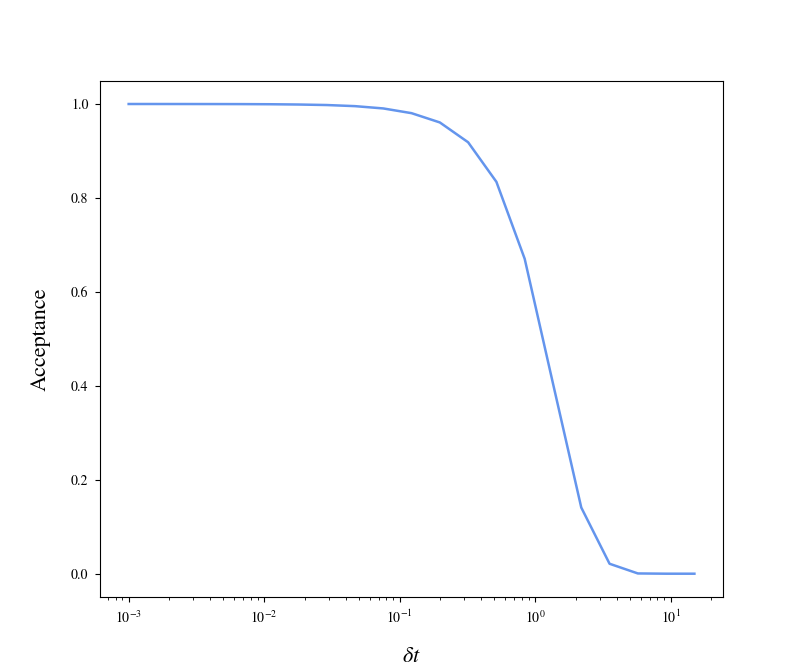
\includegraphics[scale=0.45]{images/time_steplength.png}
    \caption{Acceptance ratio as a function of the time-step $\delta t$ in the context of VMC simulation performed with the importance sampling technique. Each run is conducted with $2^{21}$ steps and involves a system of $10$ non-interacting particles in 3-dimensions with $\alpha=0.5$.  }
    \label{fig:dt_importance_sampling}
\end{figure}




\subsubsection{STATISTICAL ANALYSIS THROUGH BLOCKING METHOD}
As previously stated, Table \ref{tab:varying_alpha_noninteracting} contains estimations of the variance affecting $\langle E_L(\alpha) \rangle$ obtained directly from the variance provided by the VMC simulations and the one obtained with the Blocking technique. The python script that provided us with these latter results is based on the theoretical background described in Section \ref{sec:blocking_method}. The consistency of the mentioned script was also tested, in particular for what concerns the convergence of the evaluated variance $\sigma_\mu^2$ (see Eq.\,\ref{eq:blocking_method}) to a finite value after a sufficiently high blocking iterations. In Figure \ref{fig:blocking_analysis} we present the values of $\sigma_k$ after each iteration of the blocking method: the results are derived from a simulation performed with $2^{23}$ steps on a $3D$ system containing $N=10$ non-interacting particles inserted in a spherical potential. The sampling was performed through the Metropolis-Hastings algorithm using $\delta t=0.01$ and the variational parameter was again set to $\alpha=0.5$. As expected, we can observe that $\sigma_k$ reaches a plateau for sufficiently high values of $k$, and then an erratic behaviours enters into play, this due to the progressive reduction of the amount of points on which the variance is estimated. 

\begin{figure}[H]
    \centering
    
\includegraphics[scale=0.45]{images/yaaaa.png}
    \caption{The figure shows the behaviour of the variance estimate provided by blocking technique implemented in a python script. The simulation was performed with $2^{23}$ steps on a non-interacting $3D$ system characterized by $\alpha=0.5$ and populated by 10 particles. The Metropolis-Hastings algorithm with $\delta t =0.01$ was adopted for the sampling.}
    \label{fig:blocking_analysis}
\end{figure}


\subsection{INTERACTING CASE}
Subsequently we moved on to the interacting and asymmetrical case with trial wavefunction given by \ref{wavefunctions} and hamiltonian given by \ref{hamiltonian}. At first we compared results with those obtained from the symmetrical case, again to test the solidity of our code: this could be done by setting $\beta=1$, $w_z = w_{ho} = 1$ and the s-wave scattering length $a$ to 0. We verified that the results were coincident with those obtained in the non-interacting case, using both the Brute-force Metropolis algorithm and the importance sampling. From now on we will omit to specify the sampling algorithm used for each simulation, since all the next results were derived exploiting the Metripolis-Hastings one: this choice was driven by the fact that the this technique provides a higher acceptance ratio, corresponding to a better statistical sampling of the data. Furthermore, the variance on the energy value provided by each VMC was estimated through the blocking analysis. \\

After the aforementioned consistency check we set the parameters' values $\omega_z = \beta = 2.82843$ and $a = 0.0043$ and ran the simulations for $N=10,50,100$ particles while varying $\alpha$. All the simulations were carried out using $2^{21}$ steps and $\delta t = 0.01$: the corresponding results are reported in Tables \ref{tab:varying_alpha_interacting_10particles}, \ref{tab:varying_alpha_interacting_50particles} and \ref{tab:varying_alpha_interacting_100particles}. Furthermore, as an example the results obtained for 10 particles are reported in figure \ref{fig:asymm_symm_comparions}, compared with their homologous obtained in the non-interacting symmetrical case. Figure \ref{fig:E_over_N} reports a comparison between the energies per particle as a function of the variational parameter $\alpha$ obtained for the three different values of $N$. \\


\begin{table}[H]
    \centering
    \begin{tabular}{cccc}
        $\alpha$ & $\langle E_L \rangle$ & $\sigma_B$ & acc. ratio \\
        \midrule
        0.3 & 0 & 0 & 0 \\
        0.4 & 0 & 0 & 0 \\
        0.5 & 0 & 0 & 0 \\
        0.6 & 0 & 0 & 0 \\
        0.7 & 0 & 0 & 0 \\
    \end{tabular}
    \caption{The table reports the results of the simulations for different values of the variational parameter $\alpha$ for a $3D$ system constituted by $N=10$ particles. The simulations were performed exploiting the Metropolis-Hastings algorithm with $2^{21}$ MC steps and $\delta t=0.01$.  }
    \label{tab:varying_alpha_interacting_10particles}
\end{table}

\begin{table}[H]
    \centering
    \begin{tabular}{cccc}
        $\alpha$ & $E$ & $\sigma_B$ & $acceptance$ \\
        \midrule
        0.3 & 0 & 0 & 0 \\
        0.4 & 0 & 0 & 0 \\
        0.5 & 0 & 0 & 0 \\
        0.6 & 0 & 0 & 0 \\
        0.7 & 0 & 0 & 0 \\
        \bottomrule
    \end{tabular}
    \caption{The table reports the results of the simulations for different values of the variational parameter $\alpha$ for a $3D$ system constituted by $N=50$ particles. The simulations were performed exploiting the Metropolis-Hastings algorithm with $2^{21}$ MC steps and $\delta t=0.01$. }
    \label{tab:varying_alpha_interacting_50particles}
\end{table}

\begin{table}[H]
    \centering
    \begin{tabular}{cccc}
        $\alpha$ & $E$ & $\sigma_B$ & $acceptance$ \\
        \midrule
        0.3 & 0 & 0 & 0 \\
        0.4 & 0 & 0 & 0 \\
        0.5 & 0 & 0 & 0 \\
        0.6 & 0 & 0 & 0 \\
        0.7 & 0 & 0 & 0 \\
    \end{tabular}
    \caption{The table reports the results of the simulations for different values of the variational parameter $\alpha$ for a $3D$ system constituted by $N=100$ particles. The simulations were performed exploiting the Metropolis-Hastings algorithm with $2^{21}$ MC steps and $\delta t=0.01$. }
    \label{tab:varying_alpha_interacting_100particles}
\end{table}


\begin{figure}[H]
    
\includegraphics[scale=0.5]{images/yaaaa.png}
    \caption{}
    \label{fig:asymm_symm_comparison}
\end{figure}


\begin{figure}[H]
    
\includegraphics[scale=0.5]{images/yaaaa.png}
    \caption{Grafico a caso, plottiamo N=10, 50, 100 interagenti.}
    \label{fig:E_over_N}
\end{figure}


\subsection{GRADIENT DESCENT}

As we can see, again we found a convex function with unique minimum: this consideration allows us to perform a research for energy-minimizing parameter $\alpha^{best}$ exploiting the gradient descent method. Before proceeding with the actual investigation in the interacting case, we tested the correct functioning of our code by applying it to a non-interacting system. In this simple case, it is well known that the optimal value of the variational parameter is $\alpha=0.5$ and this result is independent of the number of particles and dimensionality of the system. Therefore we expect to reach a convergence to this value whatever is the configuration that we adopt. In particular, in this simple case of particles without interaction the analytical expression for the total energy of the system was found in Eq.\,\ref{energy_analitical} and it is easy to proof that it leads to a convex function. This ensures us that for a sufficiently small value of the so-called learning rate $\gamma$ appearing in Eq.\,\ref{alpha_k} the gradient descent will lead to a proper estimation of $\alpha_{opt}$. Table ref reports the results obtained with the application of the gradient descent method to a 3-dimensional system of 1, 10 and 100 non-interacting particles. Each VMC was performed with $\delta t=0.01$ and $10^5$ thermalization steps, followed by another $10^5$ for the actual evaluation of the quantities reported in Eq.\,\ref{dEnergy_dalpha}. The learning rate was fixed at $\gamma=0.01$ and the tolerance to $\varepsilon=10^{-5}$.


\begin{table}[H]
\centering
 \begin{tabular}{c|c|c|c|}
         & \multicolumn{3}{c|}{Importance} \\
        \hline
         Starting $\alpha$ & $\gamma$ & $N_{step}$ & Final $\alpha$ \\
       \hline
          & $0$ & $0$ & $0$ \\
         $0.4$ & $0$ & $0$ & $0$ \\
          & $0$ & $0$ & $0$ \\
         \hline
          & $0$ & $0$ & $0$ \\
         $0.6$ & $0$ & $0$ & $0$ \\
          & $0$ & $0$ & $0$ \\
         \hline
    \end{tabular}
    \caption{The table reports the results of the gradient descent method starting from $\alpha=0.4$ and $\alpha=0.6$. The simulations of the non-interacting case using a simple gaussian trial wavefunction and the Importance Sampling method. We used 10 particles in 3 dimensions and $10^5$ Monte Carlo steps. We used $10^5$ steps to thermalize the system. The timestep-size was set to $\delta t= 0.01$. }
\end{table}

\begin{table}[H]
    \centering
    \begin{tabular}{cccc}
        N & $\alpha_0$ & $\alpha_{best}$ & $N_{iterations}$ \\
        \midrule
        1 & 0.4 & ??? & ??? \\
        1 & 0.6 & ??? & ??? \\
        10 & 0.4 & ??? & ??? \\
        10 & 0.6 & ??? & ??? \\
        100 & 0.4 & ??? & ??? \\
        100 & 0.6 & ??? & ??? \\
        \bottomrule
    \end{tabular}
    \caption{Results for the energy minimization process performed on a non-interacting system of 1, 10, 100 particles in a spherical potential. The simulations were performed with $10^5$ steps for both thermalization and actual run, $\delta t = 0.01$, $\gamma=0.01$ and $\varepsilon=10^{-5}$. $N_{iterations}$ refers to the number of gradient descent steps to get to convergence.}
    \label{tab:my_label}
\end{table}


Switching now to consider the interaction between particles, in this case the problem was less trivial, since the optimal value of the variational parameter depends also on the chosen number of particles and on the starting value of $\alpha$. Moreover, contrarily to the previous case, the exact value of $\alpha_{best}$ is unknown and thus our research must me also more rigorous. The implemented method consists in a first run performed by adopting $\gamma=0.01$ for a rapid convergence to a proximity of the result we aim at ($\varepsilon=10^{-5})$, and then a finer research was started, employing $\gamma=10^{-3}$ and choosing the final tolerance to be $\varepsilon=10^{-8}$. Again the single runs were performed for $N=10$, 50 and 100 using $10^5$ VMC steps and $\delta t =0.01$. For each $N$ the research of the optimal variational parameter was performed starting from 3 initial guesses, this to verify the correctness of the result and the solidity of the algorithm. Our analysis is resumed in Table \ref{tab:gradient_descent_interacting}.

Once that the values of $\alpha_{best}$ has been achieved for any selected configuration, we proceeded with a final VMC run to estimate the ground state energy for each apparatus. The results reported in Table \ref{tab:final_GS_energy} are referred to simulations performed with $\delta t = 0.01$ and $2^{27}$ MC steps, this choice driven by the aim of increasing the accuracy in the estimation of the energy. 


\begin{table}[H]
    \centering
    \begin{tabular}{cccccc}
         & & \multicolumn{2}{c}{$\gamma=10^{-2}$} & \multicolumn{2}{c}{$\gamma=10^{-3}$} \\
         \midrule
        $N$ & $\alpha_{start}$ & $\alpha_{best}$ & $N_{steps}$ & $\alpha_{best}$ & $N_{steps}$ \\
        \midrule
        10 & 0.4 & & & & \\
        10 & 0.6 & & & & \\
        50 & 0.4 & & & & \\
        50 & 0.6 & & & & \\
        100 & 0.4 & & & & \\
        100 & 0.6 & & & & \\
        \bottomrule
    \end{tabular}
    \caption{Convergence analysis of the gradient descent method applied to a system of interacting particles. The simulations were performed using $\delta t = 0.01$ and $10^5$ MC stepsm while the tolerances have been set to $10^{-5}$ and $10^{-8}$ respectively for the case of $\gamma=0.01$ and $\gamma=10^{-3}$.}
    \label{tab:gradient_descent_interacting}
\end{table}


\begin{table}[H]
    \centering
    \begin{tabular}{ccccc}
            $N$ & $\alpha^{best}$ & $E$ & $\sigma^2_B$ & acceptance \\
            \midrule
            10 & & & &  \\
            50 &  & & &  \\
            100 &  &  &  &  \\
            \midrule
        \end{tabular}
    \caption{Results obtained for the ground state energy values computed exploiting the optimal variational parameter found after the gradient descent minimization. The simulations were performed using $\delta t = 0.01$ and $2^{27}$ steps.}
    \label{tab:final_GS_energy}
\end{table}




\subsection{ONE-BODY DENSITY}
With the energy-minimizing variational parameter at our disposal, we proceeded with the last step of our analysis, namely the evaluation of the one-body density. We limited ourselves to the deeply analyzed case of a system populated by 10 particles. Figure \ref{fig:one_body_density_histogram} shows the results obtained with the implemented procedure described in section \ref{sec:one_body_density}. For the construction of the two curves reported below, the trial wavefunction of Eq.\,\ref{wavefunctions} was considered both with and withoud the Jastrow factor and in both the cases we imposed $\alpha=\alpha_{opt}$ reported in Table \ref{tab:final_GS_energy}.


\begin{figure}[H]
    
\includegraphics[scale=0.5]{images/yaaaa.png}
    \caption{One-body density as a function of the radial distance from the center of the chosen reference frame for a $3D$ system with $N=10$ particles described by an asymmetric gaussian wavefunction and inserted in a elliptical potential. The two histograms are built respectively considering ($a\neq0$) and dropping ($a=0$) the Jastrow factor. The simulations were carried our exploiting the importance sampling with $2^{23}$ steps and $\delta t =0.01$.}
    \label{fig:one_body_density_histogram}
\end{figure}